\documentclass[11pt]{scrartcl}

\usepackage[sexy]{evan}
\usepackage{pgfplots}
\pgfplotsset{compat=1.15}
\usepackage{mathrsfs}
\usetikzlibrary{arrows}
\usepackage{graphics}
\usepackage{tikz}
\usepackage{ amssymb }
\usepackage[dvipsnames]{xcolor}
\usepackage[utf8]{inputenc}
\usepackage{longtable}
\usepackage{ragged2e}
\usepackage{listings}
\definecolor{red1}{RGB}{255, 153, 153}
\definecolor{green1}{RGB}{204, 255, 204}
\definecolor{blue1}{RGB}{204, 255, 255}
\definecolor{yellow1}{RGB}{255, 247, 160}

\definecolor{red2}{RGB}{255, 102, 102}
\definecolor{green2}{RGB}{108, 255, 108}
\definecolor{blue2}{RGB}{94, 204, 255}
\definecolor{yellow2}{RGB}{255, 250, 104}

\definecolor{red2.5}{RGB}{255,76,76}
\definecolor{green2.5}{RGB}{54, 247, 54}
\definecolor{blue2.5}{RGB}{51, 189, 255}
\definecolor{yellow2.5}{RGB}{255, 242, 52}


\definecolor{red3}{RGB}{255, 51, 51}
\definecolor{green3}{RGB}{0, 240, 0}
\definecolor{blue3}{RGB}{9, 175, 255}
\definecolor{yellow3}{RGB}{255, 234, 0}

\definecolor{red3.5}{RGB}{229, 25, 25}
\definecolor{green3.5}{RGB}{0, 194, 0}
\definecolor{blue3.5}{RGB}{4, 143, 209}
\definecolor{yellow3.5}{RGB}{255,220,0}

\definecolor{red4}{RGB}{204, 0, 0}
\definecolor{green4}{RGB}{0, 149, 0}
\definecolor{blue4}{RGB}{0, 111, 164}
\definecolor{yellow4}{RGB}{255, 206, 0}


\definecolor{noseve}{RGB}{242,242,242}

\newcommand{\camod}[1]{\frac{\ZZ}{#1 \ZZ}}
\newcommand{\modm}[1]{\text{ mod } #1}
\newcommand{\campm}[1]{\frac{\ZZ}{m\ZZ}}

\usepackage{epigraph}
\renewcommand{\epigraphsize}{\scriptsize}
\renewcommand{\epigraphwidth}{60ex}


\definecolor{dcol0}{HTML}{C8E6C9}
\definecolor{dcol1}{HTML}{D4E9B3}
\definecolor{dcol2}{HTML}{E5ED9A}
\definecolor{dcol3}{HTML}{FFF59D}
\definecolor{dcol4}{HTML}{FFE082}
\definecolor{dcol5}{HTML}{FFCC80}
\definecolor{dcol6}{HTML}{FFAB91}
\definecolor{dcol7}{HTML}{F49890}
\definecolor{dcol8}{HTML}{E57373}
\definecolor{dcol9}{HTML}{D32F2F}

\makeatletter
\newcommand{\getcolorname}[1]{dcol#1}
\makeatother

\newcommand{\dif}[1]{%
    \edef\colorindex{\number\fpeval{floor(#1)}}%
    \edef\fulltext{#1}%
    \colorbox{\getcolorname{\colorindex}}{%
        \ifnum\colorindex>8
            \textbf{\textcolor{white}{\,\fulltext\,}}%
        \else
            \textbf{\textcolor{black}{\,\fulltext\,}}%
        \fi
    }%
}
% Variable para dificultad (inicial 0)
\newcommand{\thmdifficulty}{0}

% Comando para asignar dificultad antes del problema
\newcommand{\problemdiff}[1]{\renewcommand{\thmdifficulty}{#1}}

% Estilo del problema que incluye dificultad antes del título
\declaretheoremstyle[
    headfont=\color{blue!40!black}\normalfont\bfseries,
    headformat={%
      \dif{\thmdifficulty}\quad \NAME~\NUMBER\ifx\relax\EMPTY\relax\else\ \NOTE\fi
    },
    postheadspace=1em,
    spaceabove=8pt,
    spacebelow=8pt,
    bodyfont=\normalfont
]{problemstyle}

    \declaretheorem[style=problemstyle,name=Problema,sibling=theorem]{problema}
    \declaretheorem[style=problemstyle,name=Problema,numbered=no]{problema*}

\usepackage[
backend=biber,
style=alphabetic,
sorting=ynt
]{biblatex}
\addbibresource{referencias.bib}

\title {2.- HTML (Act 2)}
\subtitle{Programación WEB I \\ Centro de Enseñanza Tecnica Industrial}
\date{20 de Agosto de 2025}
\author{Emmanuel Buenrostro 22300891 7F1}


\begin{document}

\maketitle


\begin{center}
   
\includegraphics[scale=0.15]{cetilogo.jpg} 
\end{center}
\newpage
\tableofcontents


\section{Resumen}

HTML es lo que se encarga de dar una estructura a las páginas web, lo realiza mediante distintas etiquetas que tiene disponibles, un ejemplo de estas es <h1> a <h6> que sirve para poner encabezados en la página web, o <u> que sirve para mostrar texto subrayado.


\section{Desarrollo}

\subsection{¿Qué es HTML5?}


Las siglas de HTML5 corresponden a \textbf{\textit{HyperText Markup Language}} las cuales significan:


\begin{itemize}
    \item \textbf{HyperText}, que no es más que un texto que se enlaza con otros contenidos (ya sea otros textos u otro archivo).
    Esto es la base del funcionamiento de la web, páginas y recursos interconectados.
    \item \textbf{Markup}, que significa etiqueta, ya que todas las páginas web están construidas en base a etiquetas, estas sirven para
    estructurar y definir el contenido del documento.
    \item \textbf{Language}, porque HTML es un lenguaje ya que tiene sus normas, estructuras y una serie de convenciones que nos sirven para definir
    la estructura de un sitio web. Cabe aclarar que es un lenguaje más no un lenguaje de programación ya que no cuentan con distintas estructuras como bucles, condicionales, etc.
\end{itemize}


Entonces HTML es el estándar que sirve para definir la estructura y contenido en una página web.


    \subsection{Etiquetas}


\begin{longtable}{|p{0.2\textwidth}|p{0.75\textwidth}|}
\hline
\textbf{Etiqueta} & \textbf{Función} \\
\hline
\endfirsthead
\hline
\textbf{Etiqueta} & \textbf{Función} \\
\hline
\endhead
\hline
\multicolumn{2}{|r|}{\small\textit{Continúa en la siguiente página}}\\
\endfoot
\hline
\endlastfoot
\texttt{} & Define un comentario \\
\hline
\texttt{<!DOCTYPE>} & Define el tipo de docuemento \\
\hline
\texttt{<a>} & Define un hipervínculo \\
\hline
\texttt{<abbr>} & Define una abreviación \\
\hline
\texttt{<address>} & Define la información de contacto del autor / propietario del documento \\
\hline
\texttt{<area>} & Define un área dentro de un mapa de imagen \\
\hline
\texttt{<article>} & Define un artículo \\
\hline
\texttt{<aside>} & Define el contenido lateral del contenedor de una página \\
\hline
\texttt{<audio>} & Define contenido de sonido \\
\hline
\texttt{<b>} & Define texto en negrita \\
\hline
\texttt{<base>} & Especifica la base donde se abrirán todas las URL del documento \\
\hline
\texttt{<bdi>} & Aísla una parte del texto que puede tener un formato diferente del texto externo \\
\hline
\texttt{<bdo>} & Sobreescribe la dirección del texto \\
\hline
\texttt{<blockquote>} & Define una sección que tiene otra fuente \\
\hline
\texttt{<body>} & Define el cuerpo del documento \\
\hline
\texttt{<br>} & Define un salto de línea \\
\hline
\texttt{<button>} & Define un botón clickeable \\
\hline
\texttt{<canvas>} & Se usa para dibujar gráficos en pantalla \\
\hline
\texttt{<caption>} & Define el título de una tabla \\
\hline
\texttt{<cite>} & Define el título de un trabajo \\
\hline
\texttt{<code>} & Define un trozo de código de programación \\
\hline
\texttt{<col>} & Especifica las propiedades de la columna para cada columna del elemento \texttt{<colgroup>} \\
\hline
\texttt{<colgroup>} & Especifica un grupo de una o más columnas de una tabla \\
\hline
\texttt{<command>} & Define un botón command al que un usuario puede invocar \\
\hline
\texttt{<datalist>} & Especifica en un input una lista pre-definida de opciones \\
\hline
\texttt{<dd>} & Define la descripción de un ítem en una lista de definición \\
\hline
\texttt{<del>} & Define un texto que ha sido insertado en un documento \\
\hline
\texttt{<details>} & Define detalles adicionales que el usuario puede ver o esconder \\
\hline
\texttt{<dfn>} & Define el término de una definición \\
\hline
\texttt{<dialog>} & Define una caja o ventana de dialogo \\
\hline
\texttt{<div>} & Define una sección en un documento \\
\hline
\texttt{<dl>} & Define una lista de definición \\
\hline
\texttt{<dt>} & Define un término (un ítem) en una lista de definición \\
\hline
\texttt{<em>} & Define énfasis en un texto \\
\hline
\texttt{<embed>} & Define el contenedor de una aplicación externa (no html) \\
\hline
\texttt{<fieldset>} & Grupo de elementos relacionados en un formulario \\
\hline
\texttt{<figcaption>} & Define el título para una figura \texttt{<figure>} \\
\hline
\texttt{<figure>} & Especifica auto-contenido \\
\hline
\texttt{<footer>} & Define el pie de página de un documento \\
\hline
\texttt{<form>} & Define un formulario html \\
\hline
\texttt{<h1> a <h6>} & Define encabezados o títulos \\
\hline
\texttt{<head>} & Define información acerca del documento \\
\hline
\texttt{<header>} & Define la sección de encabezado del documento \\
\hline
\texttt{<hgroup>} & Grupo de encabezado (\texttt{<h1>} a \texttt{<h6>}) \\
\hline
\texttt{<hr>} & Define un cambio de temática a partir de una línea dibujada \\
\hline
\texttt{<html>} & Define la raíz del documento \\
\hline
\texttt{<i>} & Define una parte del texto de modo alternativo \\
\hline
\texttt{<iframe>} & Define un frame en línea \\
\hline
\texttt{<img>} & Define una imagen \\
\hline
\texttt{<input>} & Define un control de entrada de texto \\
\hline
\texttt{<ins>} & Define texto que ha sido insertado en un documento \\
\hline
\texttt{<kbd>} & Define entrada del teclado \\
\hline
\texttt{<keygen>} & Define un campo generador de claves para formularios \\
\hline
\texttt{<label>} & Define el rótulo para un elemento \texttt{<input>} \\
\hline
\texttt{<legend>} & Define un título para los elementos \texttt{<fieldset>}, \texttt{<figure>}, \texttt{<details>} \\
\hline
\texttt{<li>} & Define un ítem de una lista \\
\hline
\texttt{<link>} & Define la relación entre un documento y un recurso externo (generalmente con hojas de estilo) \\
\hline
\texttt{<map>} & Define un mapa de imagen del cliente \\
\hline
\texttt{<mark>} & Define texto resaltado o marcado \\
\hline
\texttt{<menu>} & Define la lista de un menú \\
\hline
\texttt{<meta>} & Define un metadato de un documento \\
\hline
\texttt{<meter>} & Define una medida escalar en un rango conocido \\
\hline
\texttt{<nav>} & Define un link de navegación \\
\hline
\texttt{<noscript>} & Define un contenido alternativo para los usuarios que no soportan scripts del cliente \\
\hline
\texttt{<objet>} & Define un objeto embebido \\
\hline
\texttt{<ol>} & Define una lista ordenada \\
\hline
\texttt{<optgroup>} & Define un grupo de opciones relacionadas en una lista desplegable \\
\hline
\texttt{<option>} & Define una opción en una lista desplegable \\
\hline
\texttt{<output>} & Define el resultado de un cálculo \\
\hline
\texttt{<p>} & Define un párrafo \\
\hline
\texttt{<param>} & Define un parámetro para un objeto \\
\hline
\texttt{<pre>} & Define texto pre-formateado \\
\hline
\texttt{<progress>} & Representa el progreso de una tarea en una barra \\
\hline
\texttt{<q>} & Define una cita corta \\
\hline
\texttt{<rp>} & Define que debe mostrar en navegadores que no soportan scripts de ruby \\
\hline
\texttt{<rt>} & Define una pronunciación de caracteres \\
\hline
\texttt{<ruby>} & Define una notación de ruby \\
\hline
\texttt{<s>} & Define texto que no es correcto \\
\hline
\texttt{<samp>} & Define un ejemplo de salida de un programa \\
\hline
\texttt{<script>} & Define un script del lado cliente \\
\hline
\texttt{<section>} & Define una sección de un documento \\
\hline
\texttt{<select>} & Define un drop-down list \\
\hline
\texttt{<small>} & Define texto pequeño \\
\hline
\texttt{<source>} & Define los recursos para elementos multimedia \\
\hline
\texttt{<span>} & Define una pequeña sección de un documento \\
\hline
\texttt{<strong>} & Define un texto en negrita \\
\hline
\texttt{<style>} & Define un estilo para la información de un documento \\
\hline
\texttt{<sub>} & Define un texto que es subíndice \\
\hline
\texttt{<summary>} & Define un encabezado visible para el elemento \texttt{<details>} \\
\hline
\texttt{<sup>} & Define un texto que es superíndice \\
\hline
\texttt{<table>} & Define una tabla \\
\hline
\texttt{<tbody>} & Define el cuerpo de una tabla \\
\hline
\texttt{<td>} & Define una celda en una tabla \\
\hline
\texttt{<textarea>} & Define un control de entrada de múltiples líneas \\
\hline
\texttt{<tfoot>} & Agrupa los footer contenidos en una tabla \\
\hline
\texttt{<th>} & Define una celda de encabezado en una tabla \\
\hline
\texttt{<thead>} & Agrupa los encabezados de una tabla \\
\hline
\texttt{<time>} & Define fecha / hora \\
\hline
\texttt{<title>} & Define un título para el documento \\
\hline
\texttt{<tr>} & Define una fila en una tabla \\
\hline
\texttt{<track>} & Define texto de la pista para elementos multimedia (vídeo y audio) \\
\hline
\texttt{<ul>} & Define una lista desordenada \\
\hline
\texttt{<var>} & Define una variable \\
\hline
\texttt{<video>} & Define un vídeo o película \\
\hline
\texttt{<wbr>} & Define un posible salto de linea \\
\hline
\end{longtable}


\subsection{Codigo}

\lstinputlisting[language=html]{ejemplo.html}

\subsection{Captura de Pantalla}
\begin{center}
    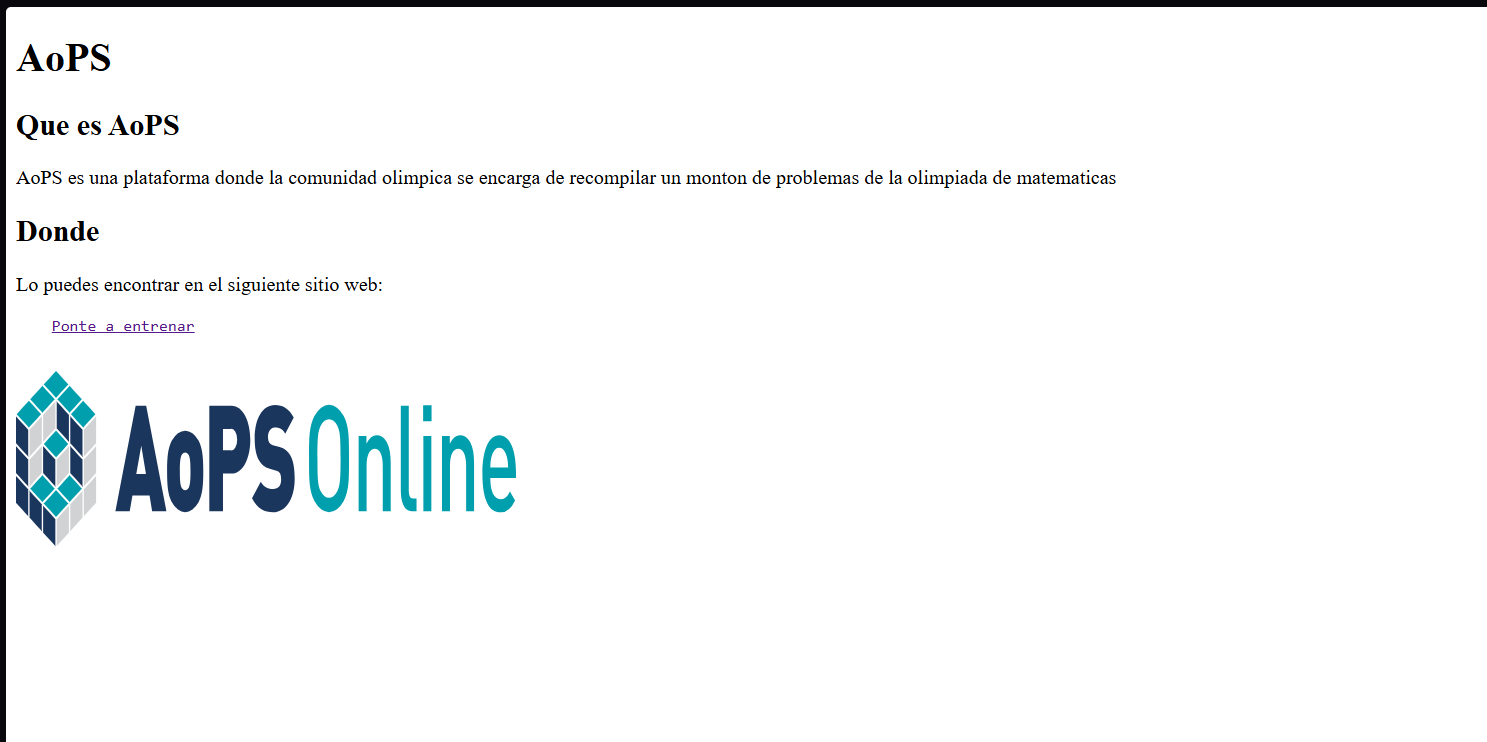
\includegraphics[scale=0.5]{CapturaSinDetalles.png}
\end{center}

\begin{center}
    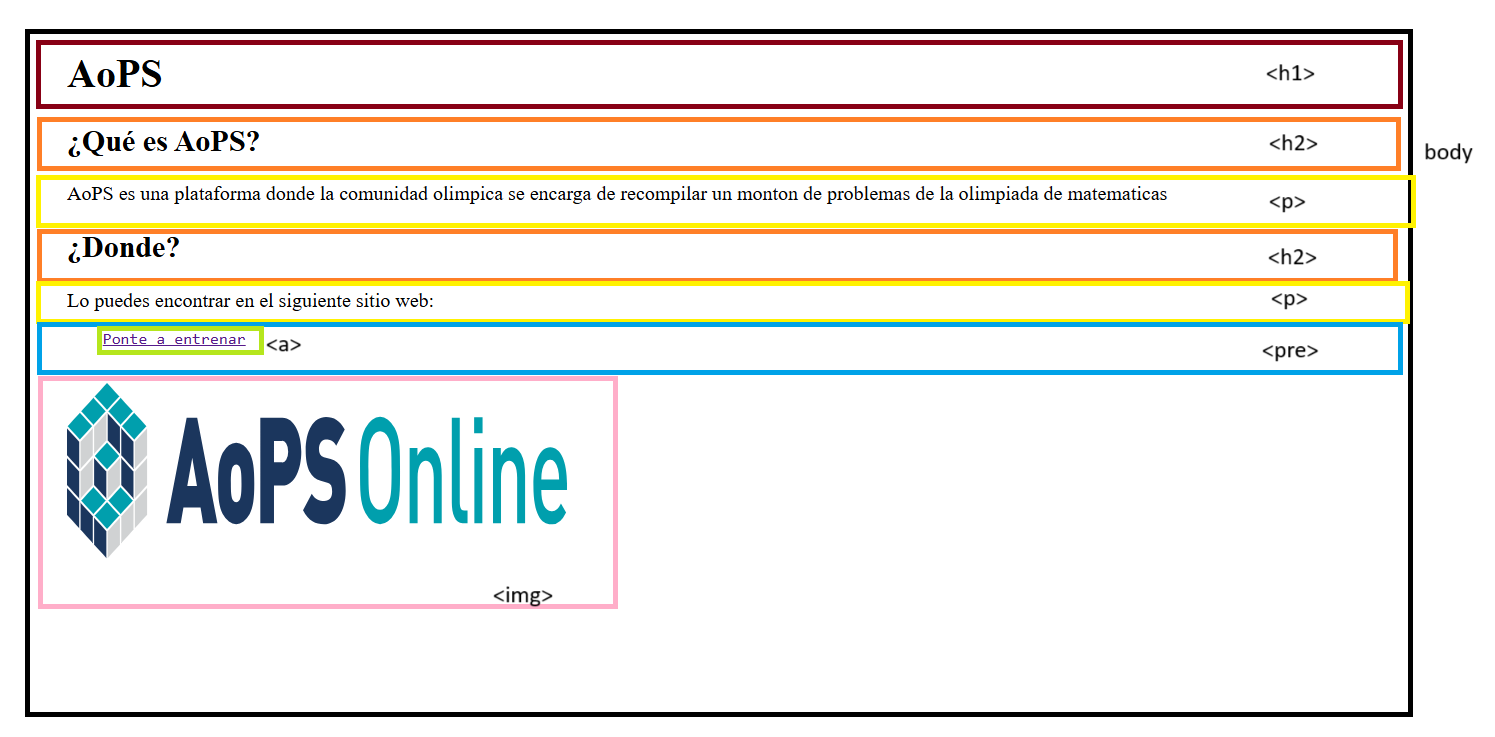
\includegraphics[scale=0.5]{CapturaHTML.png}
\end{center}


    \subsection{Actividad}

    \textbf{Pregunta: } ¿Cuál es la etiqueta para poner un texto subrayado? \\
    \textbf{Respuesta: } \texttt{<u>}
    \section{Conclusión}

    HTML es un lenguaje que tiene una lógica sencilla (hasta donde entiendo), esta actividad no tomó mucho tiempo,
    es la primera del semestre y me sentí cómodo haciéndola, además de ser algo interesante conocer un montón de etiquetas distintas que no sabía que existían.



    \section{Bibliografía}
\nocite{*}

\printbibliography[
heading=bibintoc,
title={ . }
]
    \end{document}